\documentclass{article}

\setlength{\oddsidemargin}{0.25 in}
\setlength{\evensidemargin}{-0.25 in}
\setlength{\topmargin}{-0.6 in}
\setlength{\textwidth}{6.5 in}
\setlength{\textheight}{8.5 in}
\setlength{\headsep}{0.75 in}
\setlength{\parindent}{0 in}
\setlength{\parskip}{0.1 in}

\usepackage{amsmath,amsfonts,graphicx}
\usepackage{amssymb}
\usepackage{color,xcolor}
\usepackage{minted}

% set style for the minted package
\setminted[sql]{
    breaklines=true,
    linenos=true
}

% self-defined commands
\def\ojoin{\setbox0=\hbox{\( \bowtie \)} %
    \rule[-.02ex]{.25em}{.4pt}\llap{\rule[\ht0]{.25em}{.4pt}}}
\def\leftouterjoin{\mathbin{\ojoin\mkern-5.8mu\bowtie}}
\def\rightouterjoin{\mathbin{\bowtie\mkern-5.8mu\ojoin}}
\def\fullouterjoin{\mathbin{\ojoin\mkern-5.8mu\bowtie\mkern-5.8mu\ojoin}}

\newcommand{\V}[1]{\boldsymbol{#1}}

\title{ECE 9243: Optimal and Learning Control for Robotics \\ Homework 1}
\author{Mingyu Zhao (N19569671)}

\begin{document}

\maketitle

\section*{Exercise 1: Convex optimization with linear equalities}

\subsection*{1.1 Write the Lagrangian of the optimization problem as well as the KKT conditions for optimality.}
\[ \mathcal{L}(\V{x}, \V{\lambda}) = \frac{1}{2} \V{x}^{\mathsf{T}} \V{Q} \V{x} + \V{\lambda}^{\mathsf{T}} (\V{A} \V{x} - \V{b}) \]

\subsection*{1.2 Solve the KKT system.}
Take the partial derivative with respect to \( \V{x} \) and \( \V{\lambda} \) and set them to 0:

\[ \frac{\partial \mathcal{L}}{\partial \V{x}} = 0
\ \Rightarrow \ \frac{1}{2} (\V{Q} + \V{Q^\mathsf{T}}) \V{x} + \V{A}^{\mathsf{T}} \V{\lambda} = 0
\ \Rightarrow \ \V{x} = -2 {(\V{Q} + \V{Q^\mathsf{T}})}^{-1} \V{A}^{\mathsf{T}} \V{\lambda} \]

\[ \frac{\partial \mathcal{L}}{\partial \V{\lambda}} = 0
\ \Rightarrow \ \V{A} \V{x} - \V{b} = 0 \]

Plug \( \V{x} \) into \( \V{A} \V{x} - \V{b} = 0 \):
\[ -2 \V{A} {(\V{Q} + \V{Q^\mathsf{T}})}^{-1} \V{A}^{\mathsf{T}} \V{\lambda} - \V{b} = 0
\ \Rightarrow \ \V{\lambda} = - \frac{1}{2} {(\V{A} {(\V{Q} + \V{Q^\mathsf{T}})}^{-1} \V{A}^{\mathsf{T}})} ^{-1} \V{b} \]

Plug \( \V{\lambda} \) back into the expression of \( \V{x} \):
\[ \V{x} = {(\V{Q} + \V{Q^\mathsf{T}})}^{-1} \V{A}^{\mathsf{T}} {(\V{A} {(\V{Q} + \V{Q^\mathsf{T}})}^{-1} \V{A}^{\mathsf{T}})} ^{-1} \V{b} \]

\subsection*{1.3 Use the above results to compute the minimum a function.}
Here, we have:
\[ 
\V{Q} = 
    \begin{bmatrix}
        10 & 1 & 0 \\
        1 & 100 & 2 \\
        0 & 2 & 1 
    \end{bmatrix}
\]

And the constraint:
\[ \sum_{i = 1}^{3} x_i = 1 \]

That is:
\[
\V{A} =
    \begin{bmatrix}
        1 & 1 & 1
    \end{bmatrix}
\quad b = 1
\]

Plug the value of \( \V{Q} \), \( \V{A} \) and \( b \) into the expression of \( \V{\lambda} \):
\[
\V{\lambda} = -0.89878
\quad
\V{x} =
    \begin{bmatrix}
        0.090909 & -0.010309 & 0.919400
    \end{bmatrix}
\]

Verify the constraint: \( \sum_{i = 1}^{3} x_i = 0.090909 + -0.010309 + 0.919400 = 1 \)

\section*{Exercise 2: Newton’s Method}

\subsection*{2.1 \& 2.2 Implement the Newton’s Method.}
The Newton’s method with backtracking line search is implemented in the attached Jupyter Notebook.

\subsection*{2.3 Compare the Convergence Result with the Gradient Descent Algorithm.}
As it is shown in the Jupyter Notebook, the Gradient Descent Algorithm takes 573 steps to converge for the 1D function and 75 steps for the 2D function, while the Newton’s method only takes 7 steps for the 1D function and 1 step for the 2D function. So just as proved by mathematics methods, the convergence of Newton’s method is quadratic near the minimum, which is much faster than the linear convergence of Gradient Descent algorithm.

\section*{Exercise 3: Linear Least Squares}

\subsection*{3.1 Polynomial Fitting}
Polynomial with order 3 can best fit the data. According to the plot of the error and the order, we can find out that when the order is less than 3, both training error and testing error are high, while when the order is larger than 3, both training error and testing error do not change very much. So the polynomial with order 3 is good enough for fitting this dataset without using meaningless auguments.

\begin{figure}[ht]
    \centering
    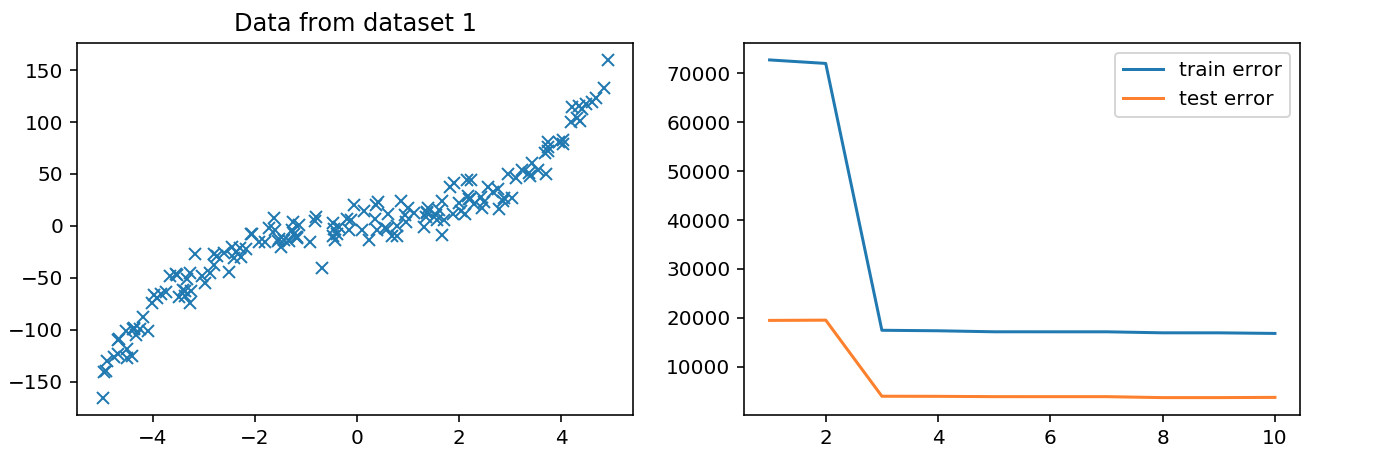
\includegraphics[width=0.8\textwidth]{imgs/1.png}
\end{figure}

And the polynomial coefficient is:
\[ a = \begin{bmatrix}
    0.72025061 & 4.67805198 & 0.05507879 & 1.0137015
\end{bmatrix}\]

The function is: 
\[ f(x) = 0.72025061 + 4.67805198 x + 0.05507879 x^2 + 1.0137015 x^3 \]

Plot this function and the data from the dataset, and it looks good:
\begin{figure}[ht]
    \centering
    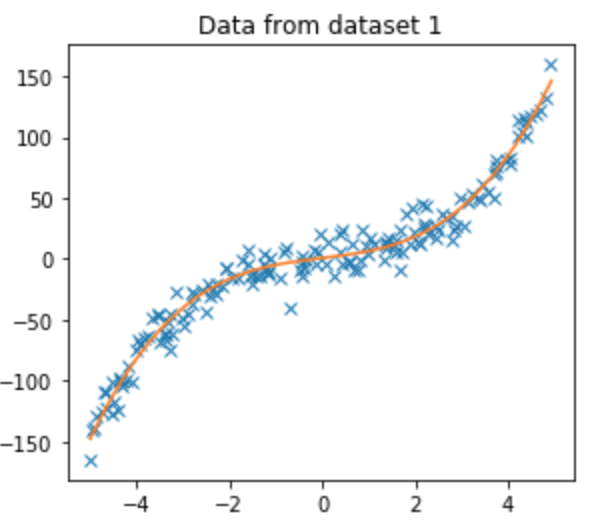
\includegraphics[width=0.4\textwidth]{imgs/2.png}
\end{figure}

\subsection*{3.2 Fit with Periodic Functions}

\subsubsection*{3.2.1 Write down the optimization problem that allows to find the coefficients.}

First, write down the optimization problem, suppose we have dataset which contains \( X \) and \( Y \):
\[ X = 
    \begin{bmatrix} 
        x_{0,1}& x_{0,2} \\
        x_{1,1}& x_{1,2} \\
        \vdots&\vdots \\
        x_{N-1,1}& x_{N-1,2}
    \end{bmatrix}
\quad
Y = \begin{bmatrix} y_0 \\ y_1 \\ \vdots \\ y_{N-1} \end{bmatrix} \]

Then, in order to find \( a_k \) and \( b_k \), we need optimize:
\[ \min\limits_{a_0, \ldots, a_K \ b_1, \ldots, b_K} 
    \sum_{i=0}^{N-1} {\bigg(a_0 + \sum_{k=1}^K \Big(a_k \cos(k T 2 \pi X_{i,k}) + b_k \sin(k T 2 \pi X_{i,k})\Big) - Y_i\bigg)}^2 \]

Let 
\[ W = 
\begin{bmatrix} 
    1 & \cos(T 2 \pi X_{0,1}) & \cdots & \cos(K T 2 \pi X_{0,K}) & \sin(T 2 \pi X_{0,1}) \cdots & \sin(K T 2 \pi X_{0,K}) \\
    1 & \cos(T 2 \pi X_{1,1}) & \cdots & \cos(K T 2 \pi X_{1,K}) & \sin(T 2 \pi X_{1,1}) \cdots & \sin(K T 2 \pi X_{1,K}) \\
    \vdots & \vdots & \vdots & \vdots & \vdots & \vdots  \\
    1 & \cos(T 2 \pi X_{N-1,1}) & \cdots & \cos(K T 2 \pi X_{N-1,K}) & \sin(T 2 \pi X_{N-1,1}) \cdots & \sin(K T 2 \pi X_{N-1,K})
\end{bmatrix} \]

As well as the parameters:
\[ \V{a} =
    \begin{bmatrix}
        a_0 \\
        a_1 \\
        \vdots \\
        a_K \\
        b_1 \\
        \vdots \\
        b_K
    \end{bmatrix} \]

So that we can simplified the lose function:
\[ L(\V{a}) = 
    {(W \V{a} - Y)}^{\mathsf{T}} (W \V{a} - Y) \]

The original problem can be rewrite as:
\[ \min\limits_{\V{a}} {(W \V{a} - Y)}^{\mathsf{T}} (W \V{a} - Y) \]

which is equal to
\[ \min_{\V{a}} {\V{a}}^{\mathsf{T}} W^{\mathsf{T}} W \V{a} - 2 Y^{\mathsf{T}} W \V{a} + Y^2 \]

which is a convex function, so the necessary and sufficient conditions to find the minimum of the function is to find the value of \( \V{a} \) that makes the gradient 0:
\[ \frac{\partial L}{\partial \V{a}} = \left(\V{a}^\mathsf{T} X^\mathsf{T} W \V{a} - 2 Y^\mathsf{T} W \V{a} + Y^2 \right) = 2 W^\mathsf{T} W a - 2W^\mathsf{T} Y = 0 \]

If the matrix \( W^\mathsf{T}W \) is invertable, then the solution to the problem is
\[ \V{a} = {(W^\mathsf{T} W)}^{-1} W^\mathsf{T} Y \]

\subsubsection*{3.2.2 Implement a function that solves the problem for periodic functions.}
This function is implemented in Jupyter Notebook as \textbf{do\_regression\_with\_periodic ()}.

\subsubsection*{3.2.3 Find the best fit for the data stored in the file regression\_dataset2.}
In this particular case that \( K = T = 1 \), so \( f(x) = a_0 + a_1 \cos(2 \pi x) + b_1 \sin(2 \pi x) \). We need to minimize:
\[ L(a_0, a_1, b_0) = \sum_{i=0}^{N-1} {(a_0 + a_1 \cos(2 \pi X_i) + b_1 \sin(2 \pi X_i) - Y_i)}^2 \]

Let
\[
    \V{a} = 
    \begin{bmatrix}
        a_0 \\
        a_1 \\
        b_1
    \end{bmatrix}
    \quad
    W = 
    \begin{bmatrix} 
        1 & w_{0,1} & w_{0,2} \\
        1 & w_{1,1} & w_{1,2} \\
        \vdots & \vdots & \vdots \\
        1 & w_{N-1,1} & w_{N-1,2}
    \end{bmatrix}
    =
    \begin{bmatrix} 
        1 & \cos(2 \pi X_0) & \sin(2 \pi X_0) \\
        1 & \cos(2 \pi X_1) & \sin(2 \pi X_1) \\
        \vdots & \vdots & \vdots \\
        1 & \cos(2 \pi X_{N-1}) & \sin(2 \pi X_{N-1})
    \end{bmatrix}
\]

So we can derive the closed-form solution:
\[ \V{a} = {(W^\mathsf{T} W)}^{-1} W^\mathsf{T} Y \] 

And I can provide more details of implementation in the Jupyter Notebook.

\subsubsection*{3.2.4 Plot the fitting function and the data from the dataset.}
Plot this function and the data from the dataset, and it looks not good enough but it is limited by the setting of \( K \) and \( T \). In this case, the loss function is already minimized:
\begin{figure}[ht]
    \centering
    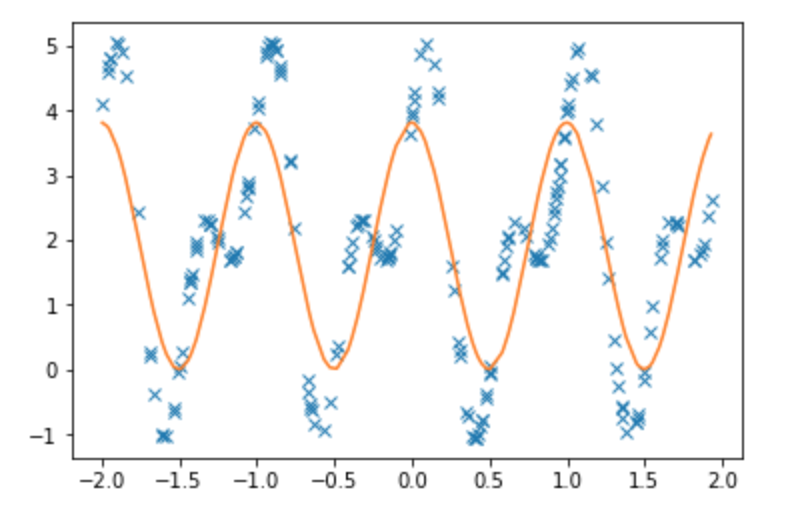
\includegraphics[width=0.5\textwidth]{imgs/3.png}
\end{figure}

As a result, I tried to change \( K \) into 2, while using the same \( x \) for each \( x_k \) to reconstruct the \( \V{W} \). Here is the fitting result, and it looks good:
\begin{figure}[ht]
    \centering
    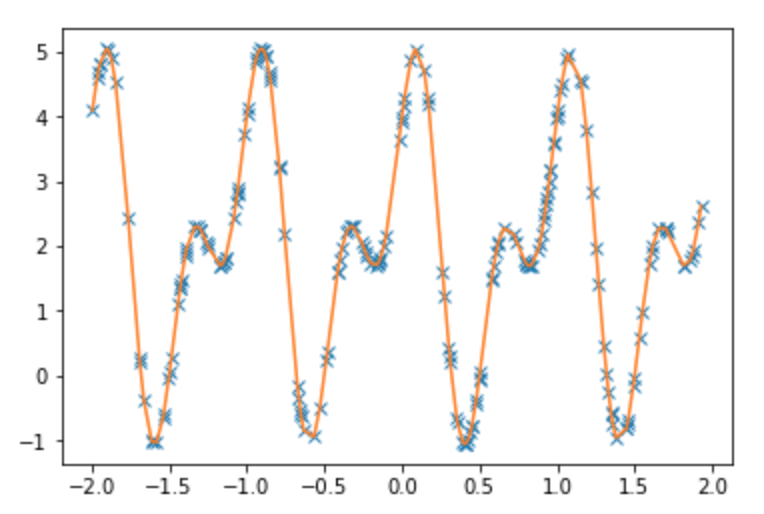
\includegraphics[width=0.5\textwidth]{imgs/4.png}
\end{figure}

\end{document}
